

\section{Data Dissemination}

In addition to extracing and organizing the dataset, we designed a web application with which a user can browse and visualize the data on-demand. The user can download various versions of the dataset and visualize the political variables spatio-temporally. Keeping scalability and consistent user experience in mind, LokDhaba is implemented with a model-view-controller architecture. The tables described in the previous section are converted into an SQL database that provides the model. This database is exposed through a Python API, and a React-based framework is used for fast rendering of visualizations with client-side filtering.

%The whole system is composed in docker with db, api and react node as independent interlinked services. 

The main ways for an end-user to interact with the data are the following:
\begin{itemize}
    \item \textbf{Browse and Download Data}: the user can explore and download the dataset online.
    \item \textbf{Data Visualization}: the user can build charts and maps to visualize election results from a political science perspective.
    \item \textbf{Incumbency profile}: the user can explore the career performance of election candidates using a novel visualization interface.
\end{itemize}

\subsection{Data Preparation}

The front-end access to LokDhaba is characterized by read-only operations. LokDhaba uses a MySQL database to store and retrieve data efficiently. Pre-computed tables are stored for assembly, constituency, party and candidate level tables to provide quick visualizations in the front-end.

%This database is executed as a separate docker service which gets initialized with empty tables whenever the service is build. This design implementation of database helps keeps us away from managing databases and related issues with security, performance, safety, resource utilization and availability.

An API based on representational state transfer architecture (REST) is implemented in Python as the interface between the React-based front-end and the database. Various pieces of functionality are designed as React ``routes'' to get data for different visualization inputs, constituency boundaries, paginated browsing and download. The API receives inputs from the user interface via POST requests, creates parameterized SQL queries to extract data from the database, and sends it back as JSON objects.  

\subsection{User Interface}

The main components for the user interface are as follows.
 
\subsubsection{Browse and Download Data}
 
 While LokDhaba incorporates several visualizations, it is important to enable users to download the raw or filtered datasets to perform their own analysis. It is also important for users to zoom in to a specific row in the table if they are interested in a particular election, or a particular candidate, etc. The Browse and Download component is designed for viewing, filtering, and sorting raw data for any election. The user selects election type and state name, and multiple assemblies of the selected state to view election results. She can also download raw data, filtered down based on any criteria, as a comma separated values (CSV) file. This component uses a \emph{react-table} component to render a large number of rows as a paginated table. It also supports quick, client-side filtering and sorting.
 
 Fig.~\ref{browse} shows a screenshot of the browse data component with results for the 2019 Parliamentary elections. Note that the position is filtered to 1, so as to list only winning candidates. Users can also filter by any other value on different columns.
  
 \begin{figure}
 \centering
 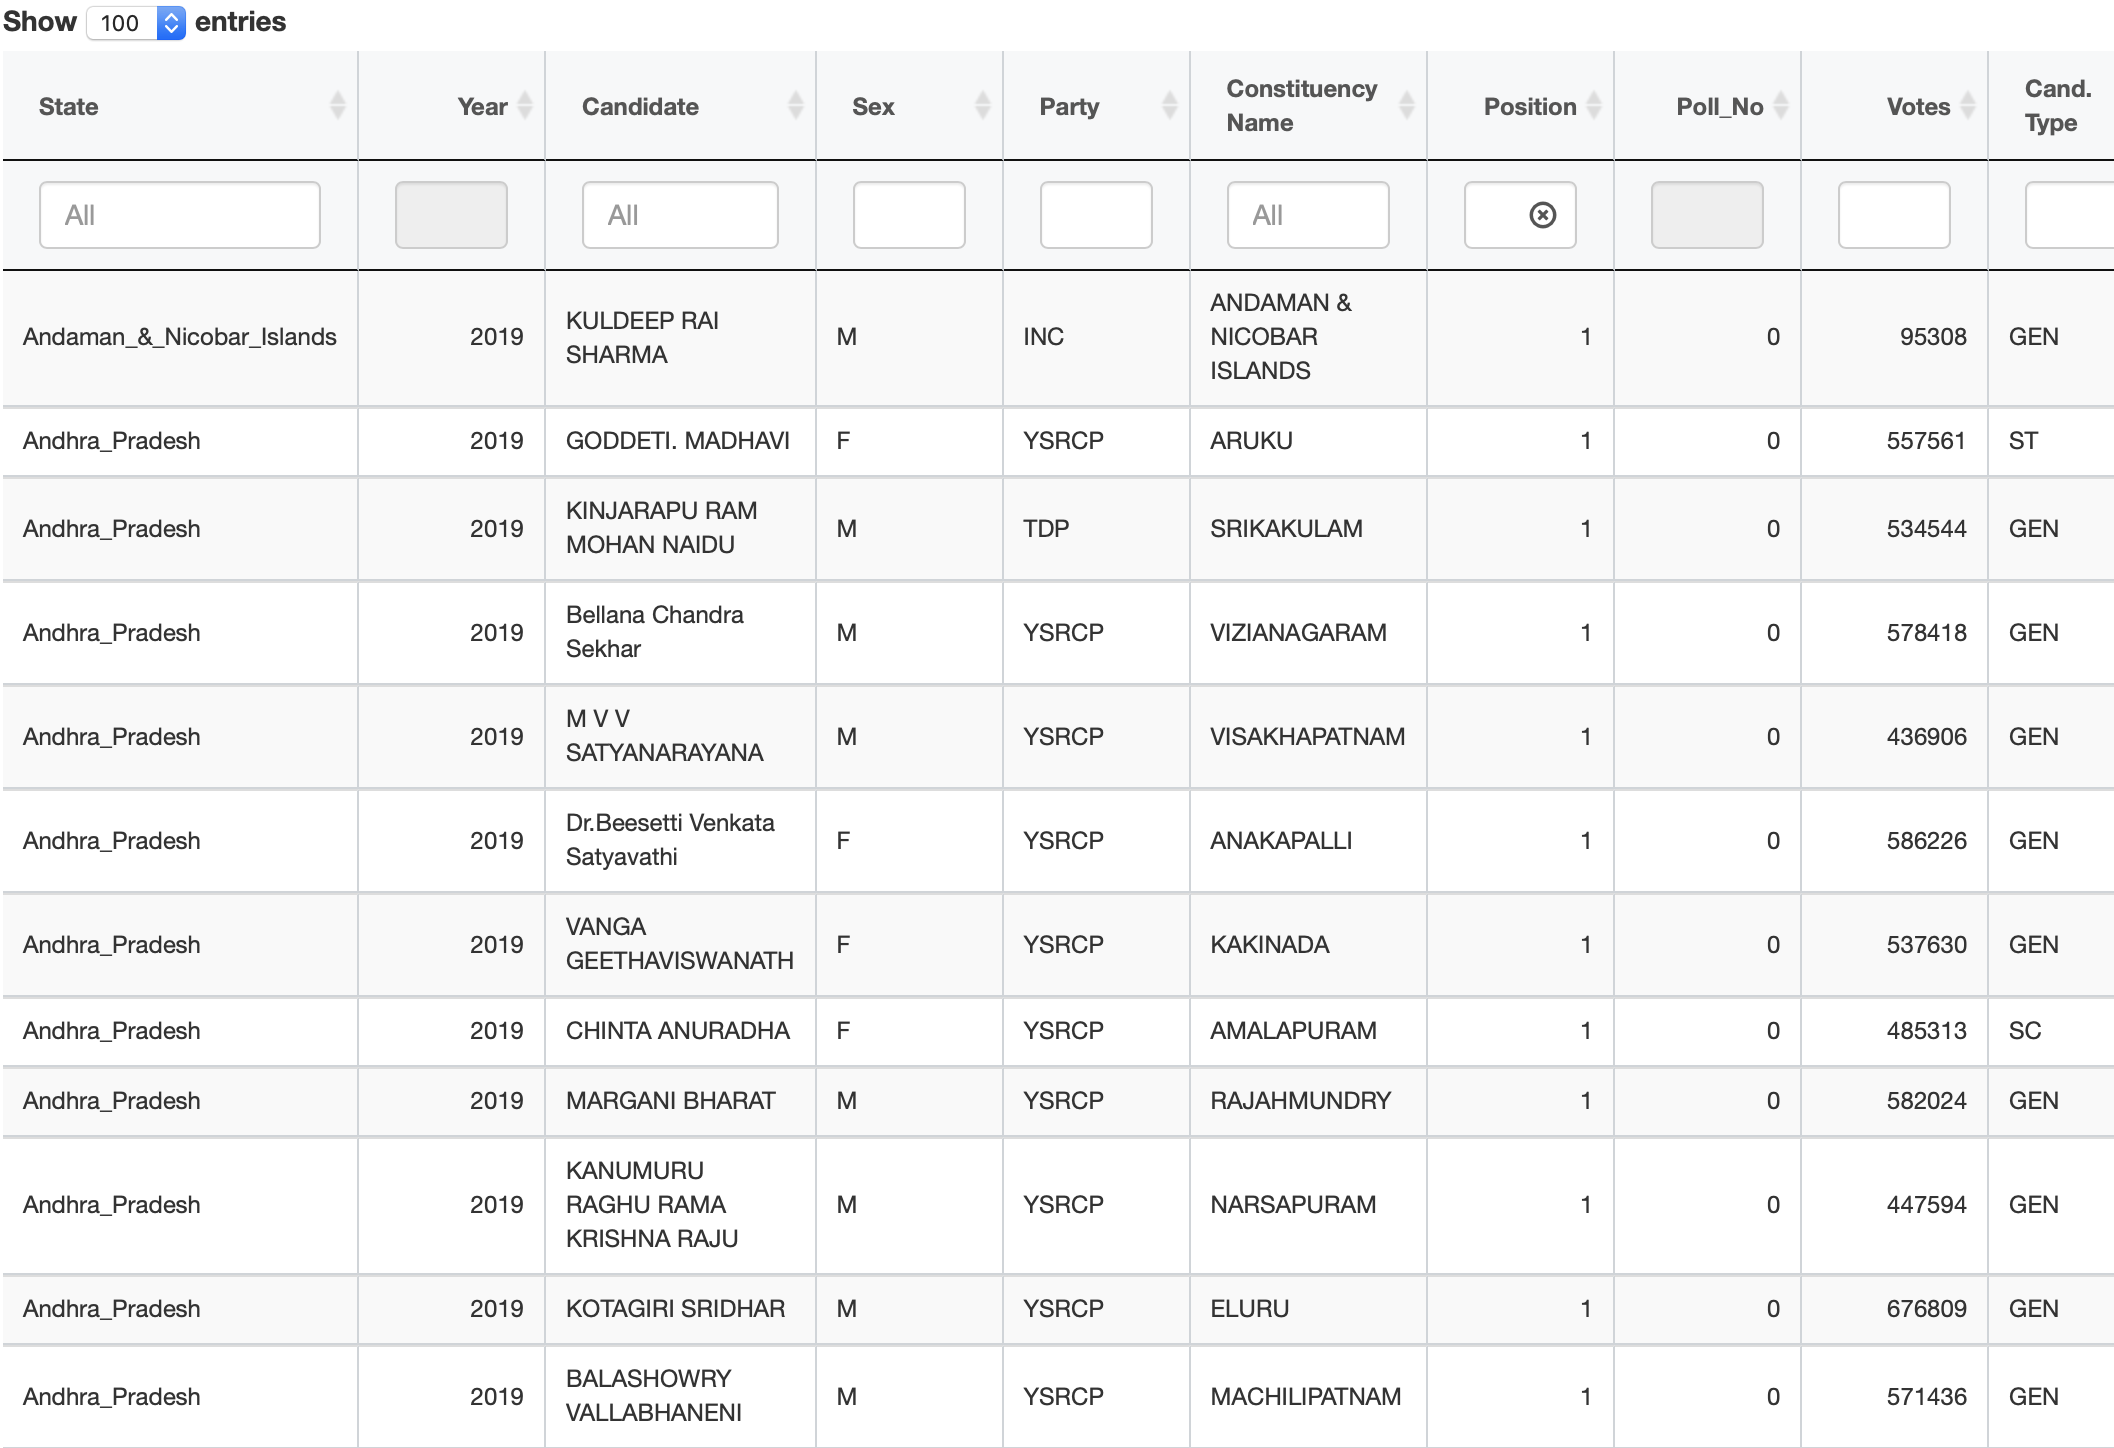
\includegraphics[width=\linewidth]{BrowseLS17Winners}
 \caption{Browse data to show all position 1 candidates of the 2019 Parliamentary election}
%%  \Description{browse ls17 winners}
 \label{browse}
 \end{figure}
 
 \subsubsection{Data Visualization}
  To implement visualizations in LokDhaba, we interviewed political scientists and analyzed media reports to see which visualizations would be the most useful. Based on this analysis, we designed the following time-line charts and visualizations which can be created on-demand by the user for any set of elections.

\begin{enumerate}
    \item \textbf{Voter turnout}: male, female and total voter turnout percentages.
    \item \textbf{Party vote share (contested)}: vote share percentage of main parties for seats they contested. (Not all parties contest all seats, especially in the presence of seat-sharing agreements.)
    \item \textbf{Party vote share (all seats)}: vote share percentage of the main parties across all seats.
    \item \textbf{Party seat share}: seat share percentage of the main parties.
    \item \textbf{Parties contested and represented}: number of parties that contested and number of parties that got at least one candidate elected.
    \item \textbf{Candidates contested/deposit lost}: number of candidates who contested the election and number of candidates who lost their deposits.
\end{enumerate}

To enable spatial exploration of election results, we came up with the following set of maps\footnote {As shape files for pre-2008 elections are not available, the current version of LokDhaba has maps only for elections post-2008.}. The maps fall into two basic categories: heat maps showing the intensity of a variable (e.g., vote share of a party), and categorical maps used to indicate spatial distribution (e.g., winning party across space).

\begin{enumerate}
    \item \textbf{Constituency type}: different colors for constituency type, a field which can be one of (1) General (open for any one to contest), (2) SC (scheduled caste candidates only) or (3) ST (scheduled tribe candidates only).
    \item \textbf{Number of candidates}: a heat map showing number of candidates contesting in each constituency.
    \item \textbf{Voter turnout}: a heat map of the voter turnout percentage in each constituency.
    \item \textbf{Winners by party}: party-wise coloring for the winning party in each constituency. Parties are mapped to color that are naturally associated with them, using a small color mapping file.
    \item \textbf{Winners by gender}: gender-wise coloring for the winner in each constituency.
    \item \textbf{Victory margin}: a heat map of the difference between the winner and first runner-up in each constituency.
    \item \textbf{Vote share of winners}: a heat map of the vote share percentage of the winner in each constituency.
    \item \textbf{Party-wise positions}: a heat map of the rank of the specified party's candidates in each constituency.
    \item \textbf{Party-wise vote share}: a heat map of the vote share percentage of the specified party's candidates in each constituency.
    \item \textbf{NOTA vote}: a heat map of the NOTA (None of the Above) vote share percentage in each constituency.
\end{enumerate}

  The data visualization component is designed to visualize aggregated statistics at a temporal or spatial level. The user selects election type, state name, visualization, and visualization specific variables to be charted or mapped. The individual visualization components take returned data from the API to render charts in \emph{react-plotly} and maps in \emph{react-leaflet}.
 
 Some screenshots of the visualization components are shown in Figs. \ref{partyCR} to \ref{partyWn}. Fig. \ref{partyCR} shows the timeline of parties contested and parties represented over all national assembly assemblies as a bar chart. Fig. \ref{partyVS} shows the vote shares of the ``main'' parties\footnote{Parties in the top two positions by seat share in any previous election.}.

  Figure \ref{BJPVS} shows a heat map of vote shares of candidates from the BJP party in the 17th Parliamentary elections. Fig. \ref{partyWn} shows the constituencies of elected members to the 17th Parliament, color coded by party.
 \begin{figure}
  \centering
  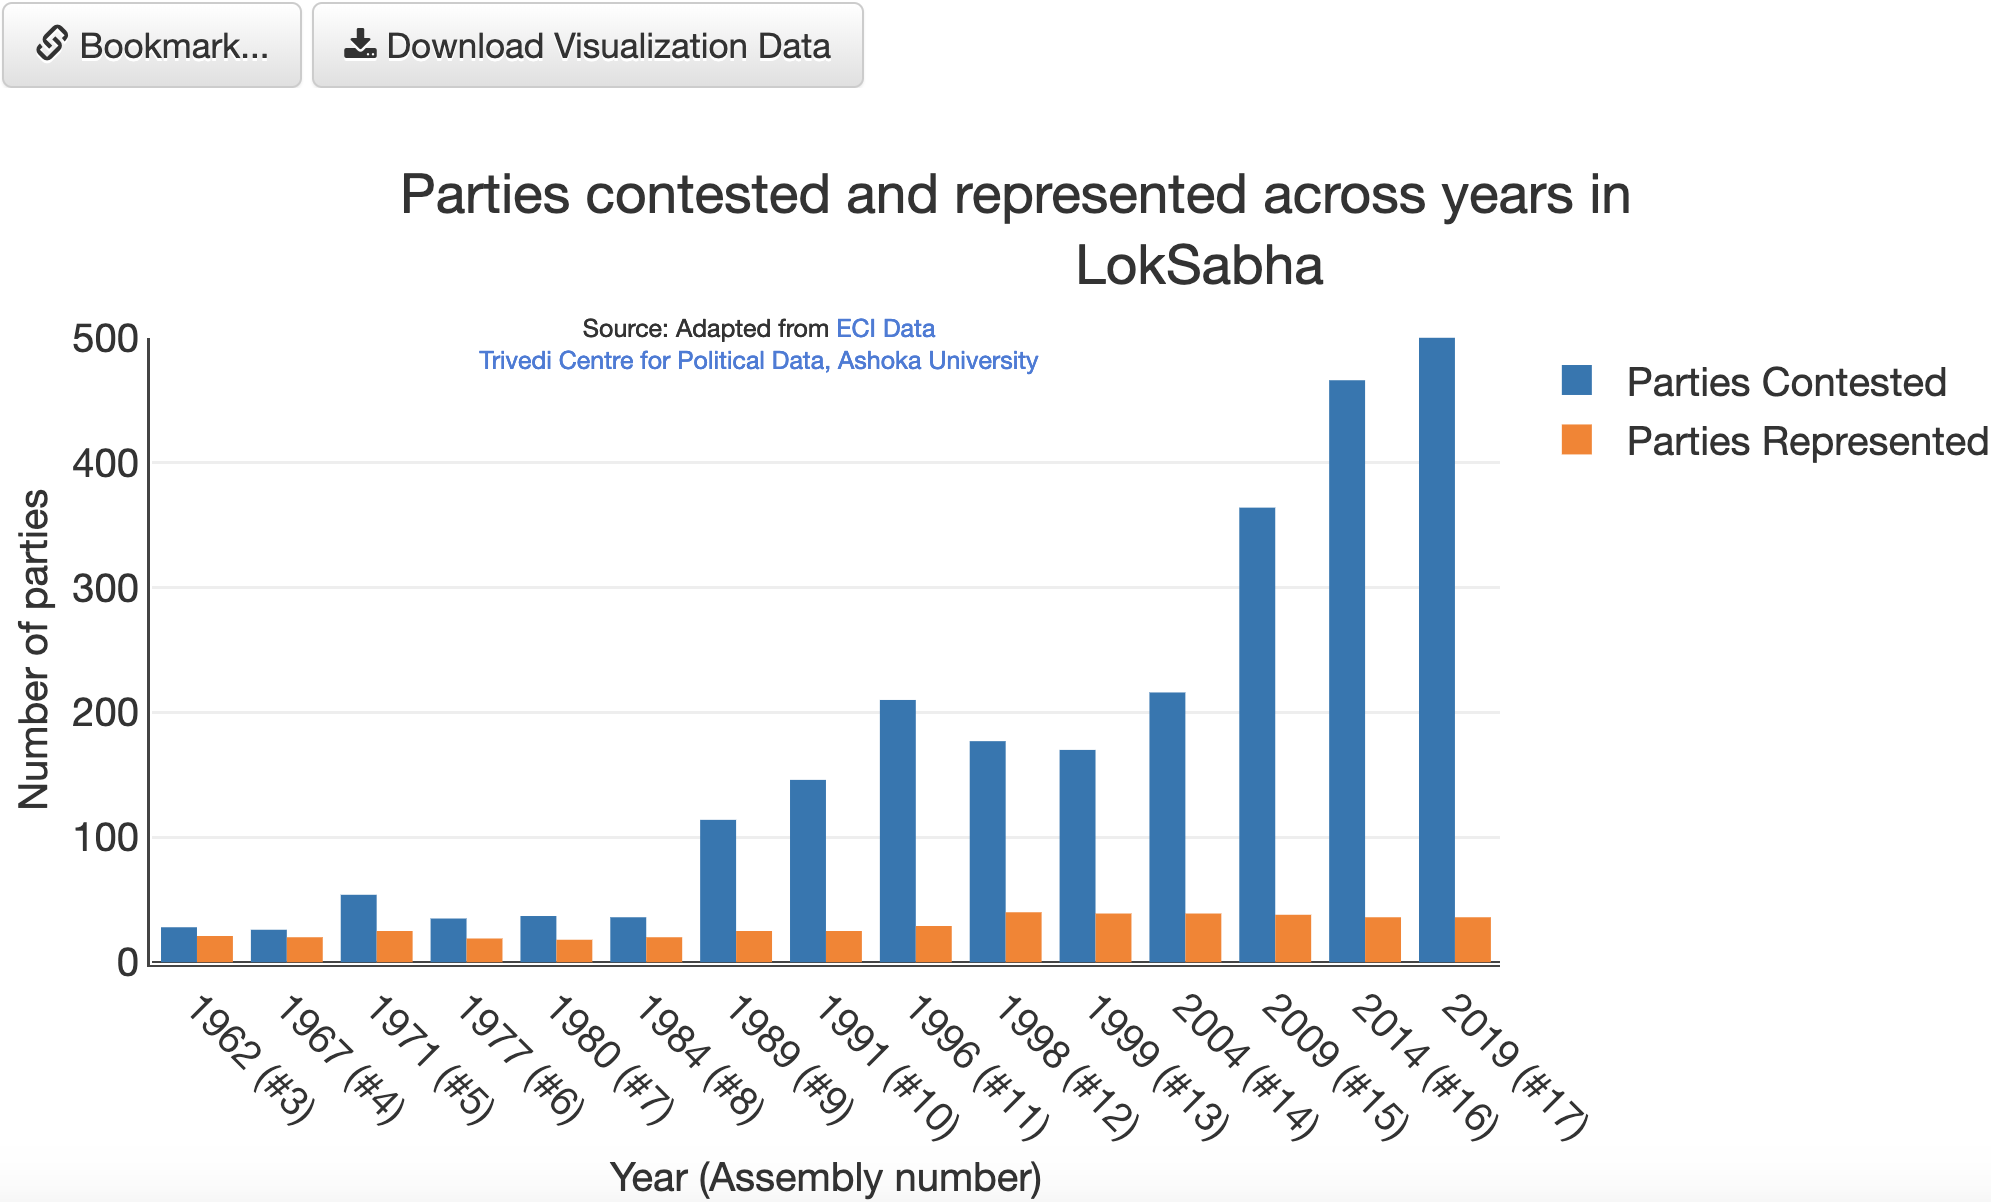
\includegraphics[width=\linewidth]{partiesContestedRepresented}
  \caption{LokDhaba visualization of parties contested and represented in national elections}
  \label{partyCR}
  \end{figure}
  
  \begin{figure}
  \centering
  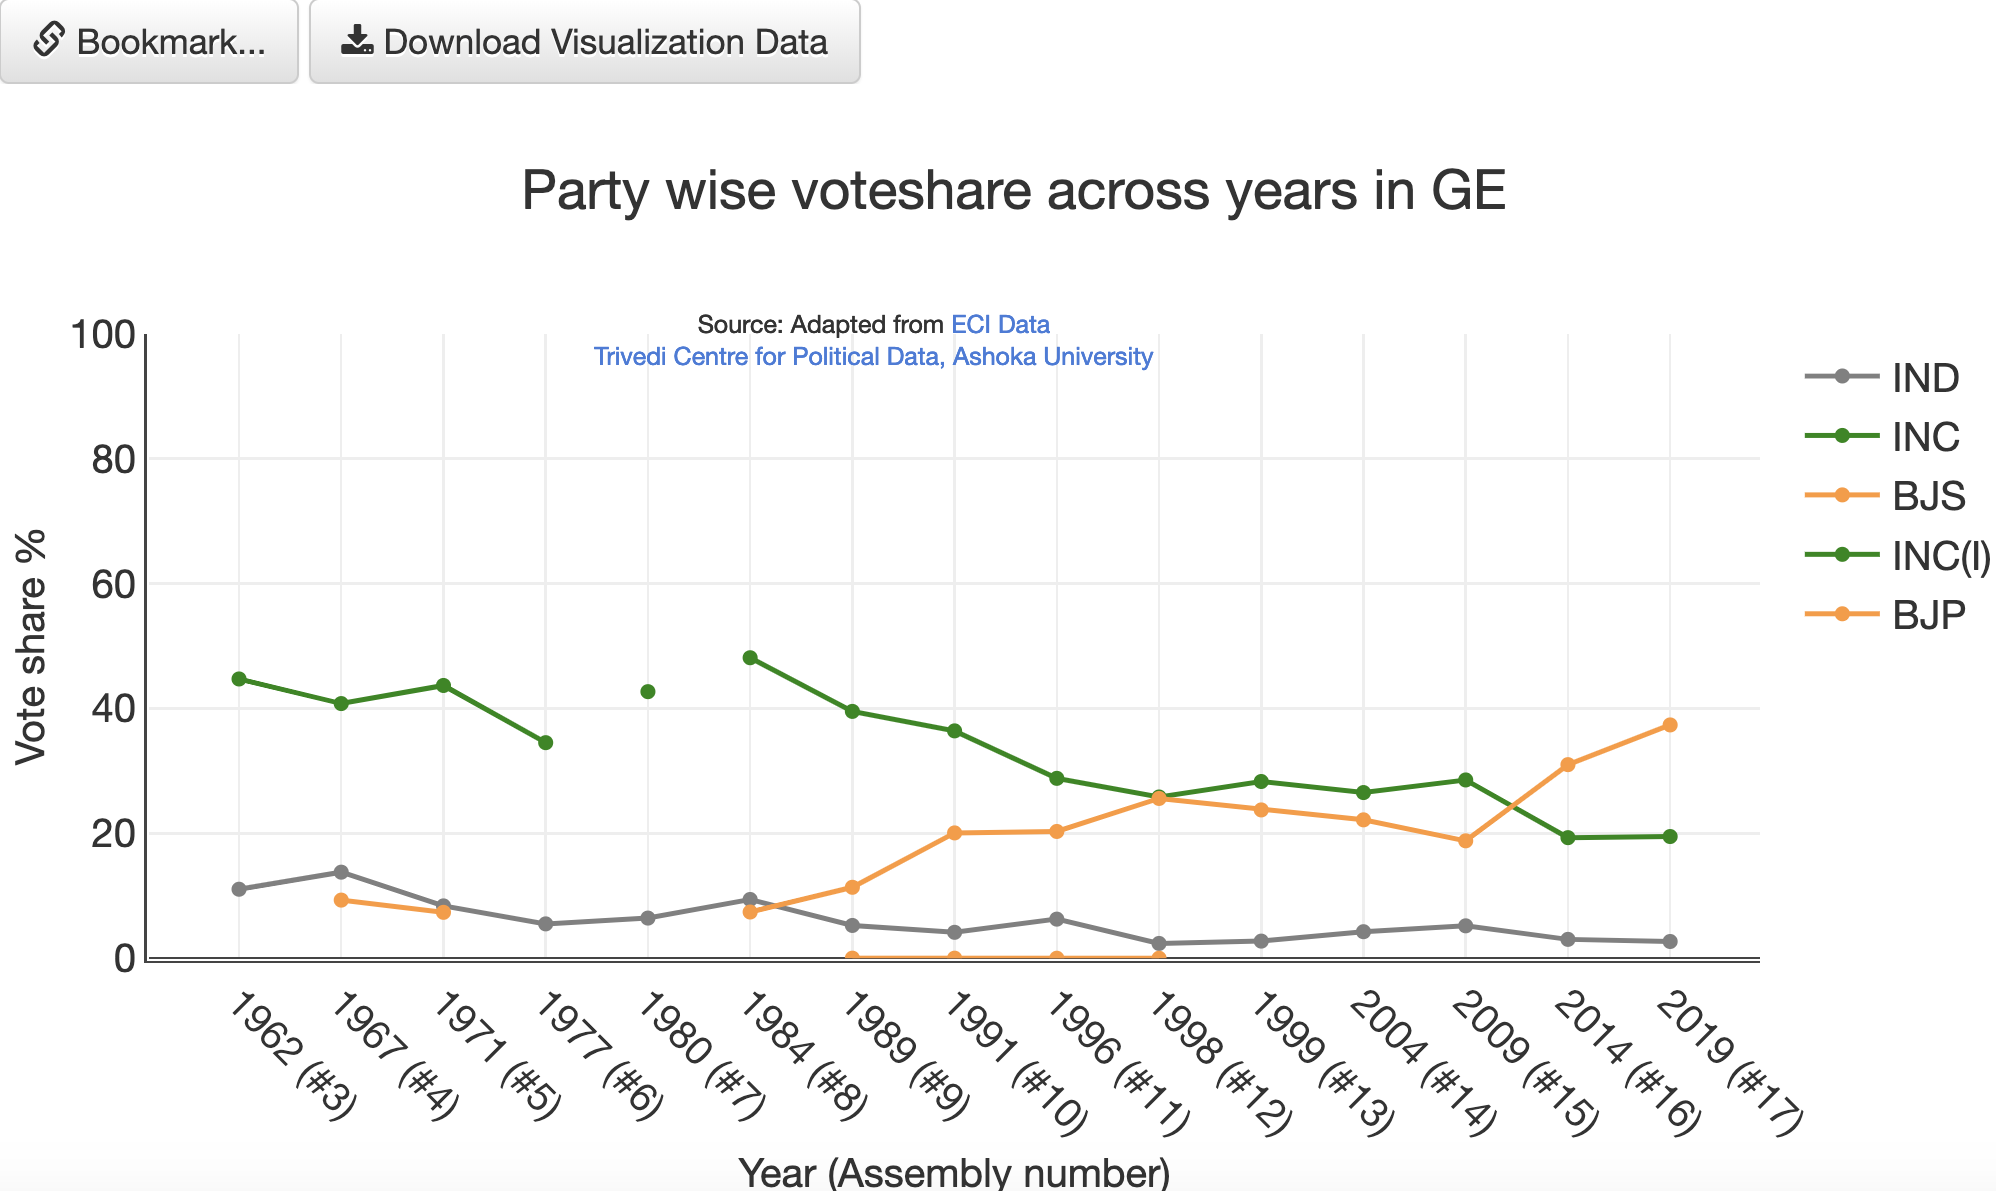
\includegraphics[width=\linewidth]{partyVoteShareTimeline}
  \caption{LokDhaba visualization of party vote shares in national elections}
  \label{partyVS}
  \end{figure}

 \begin{figure}
 \centering
 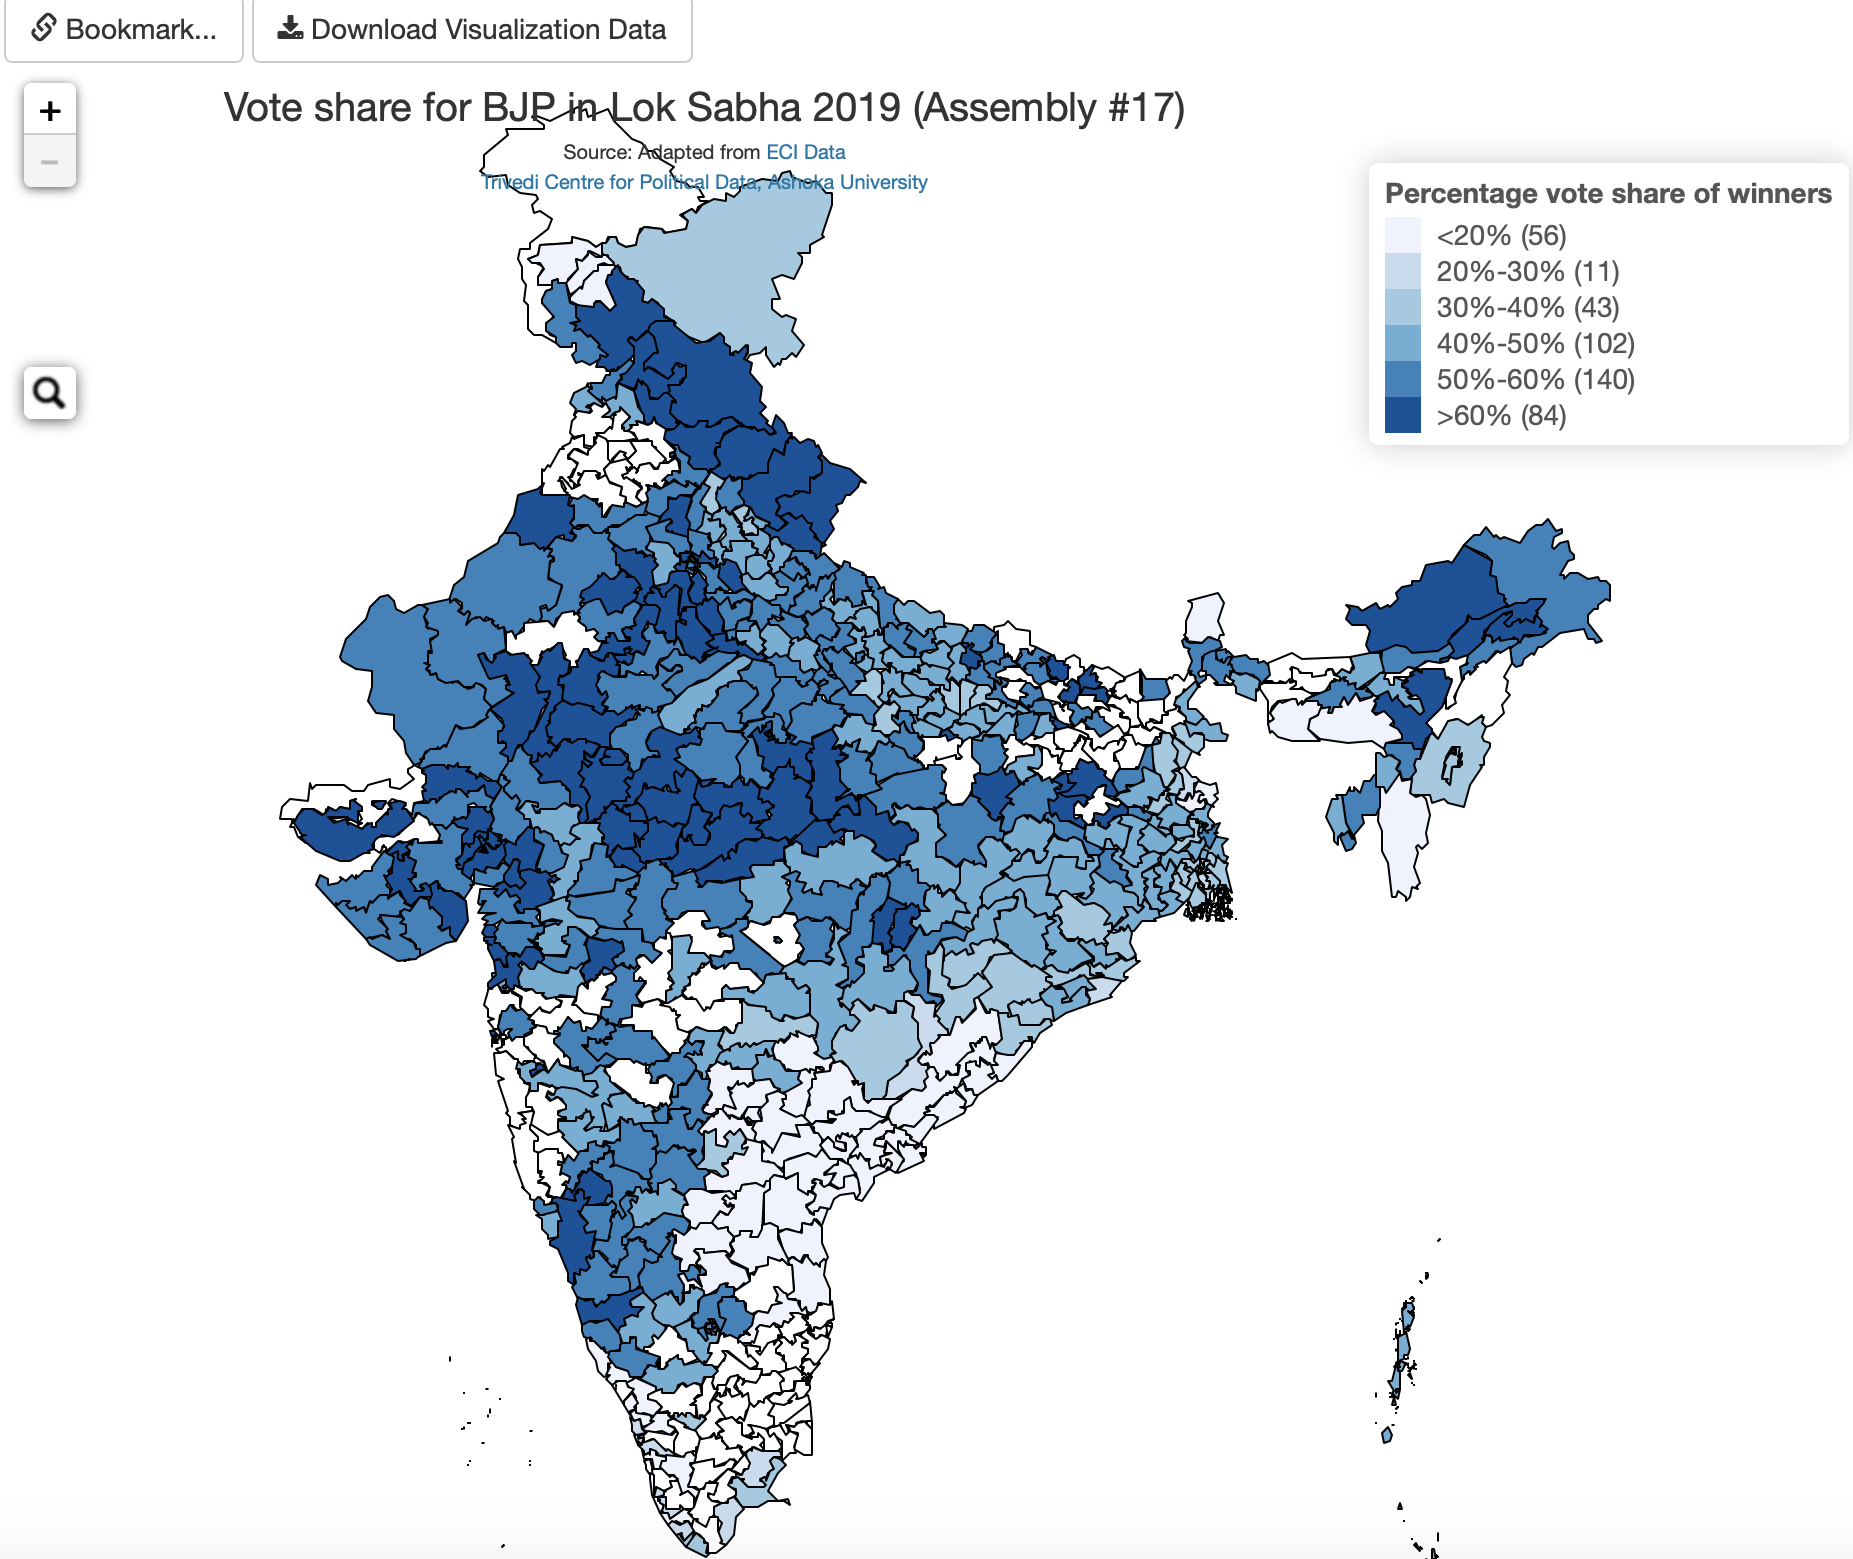
\includegraphics[width=\linewidth]{BJPVoteshare2019}
 \caption{Visualization of constituency-wise vote shares of BJP candidates in the 2019 national elections}
 \label{BJPVS}
 \end{figure}
 
 \begin{figure}
 \centering
 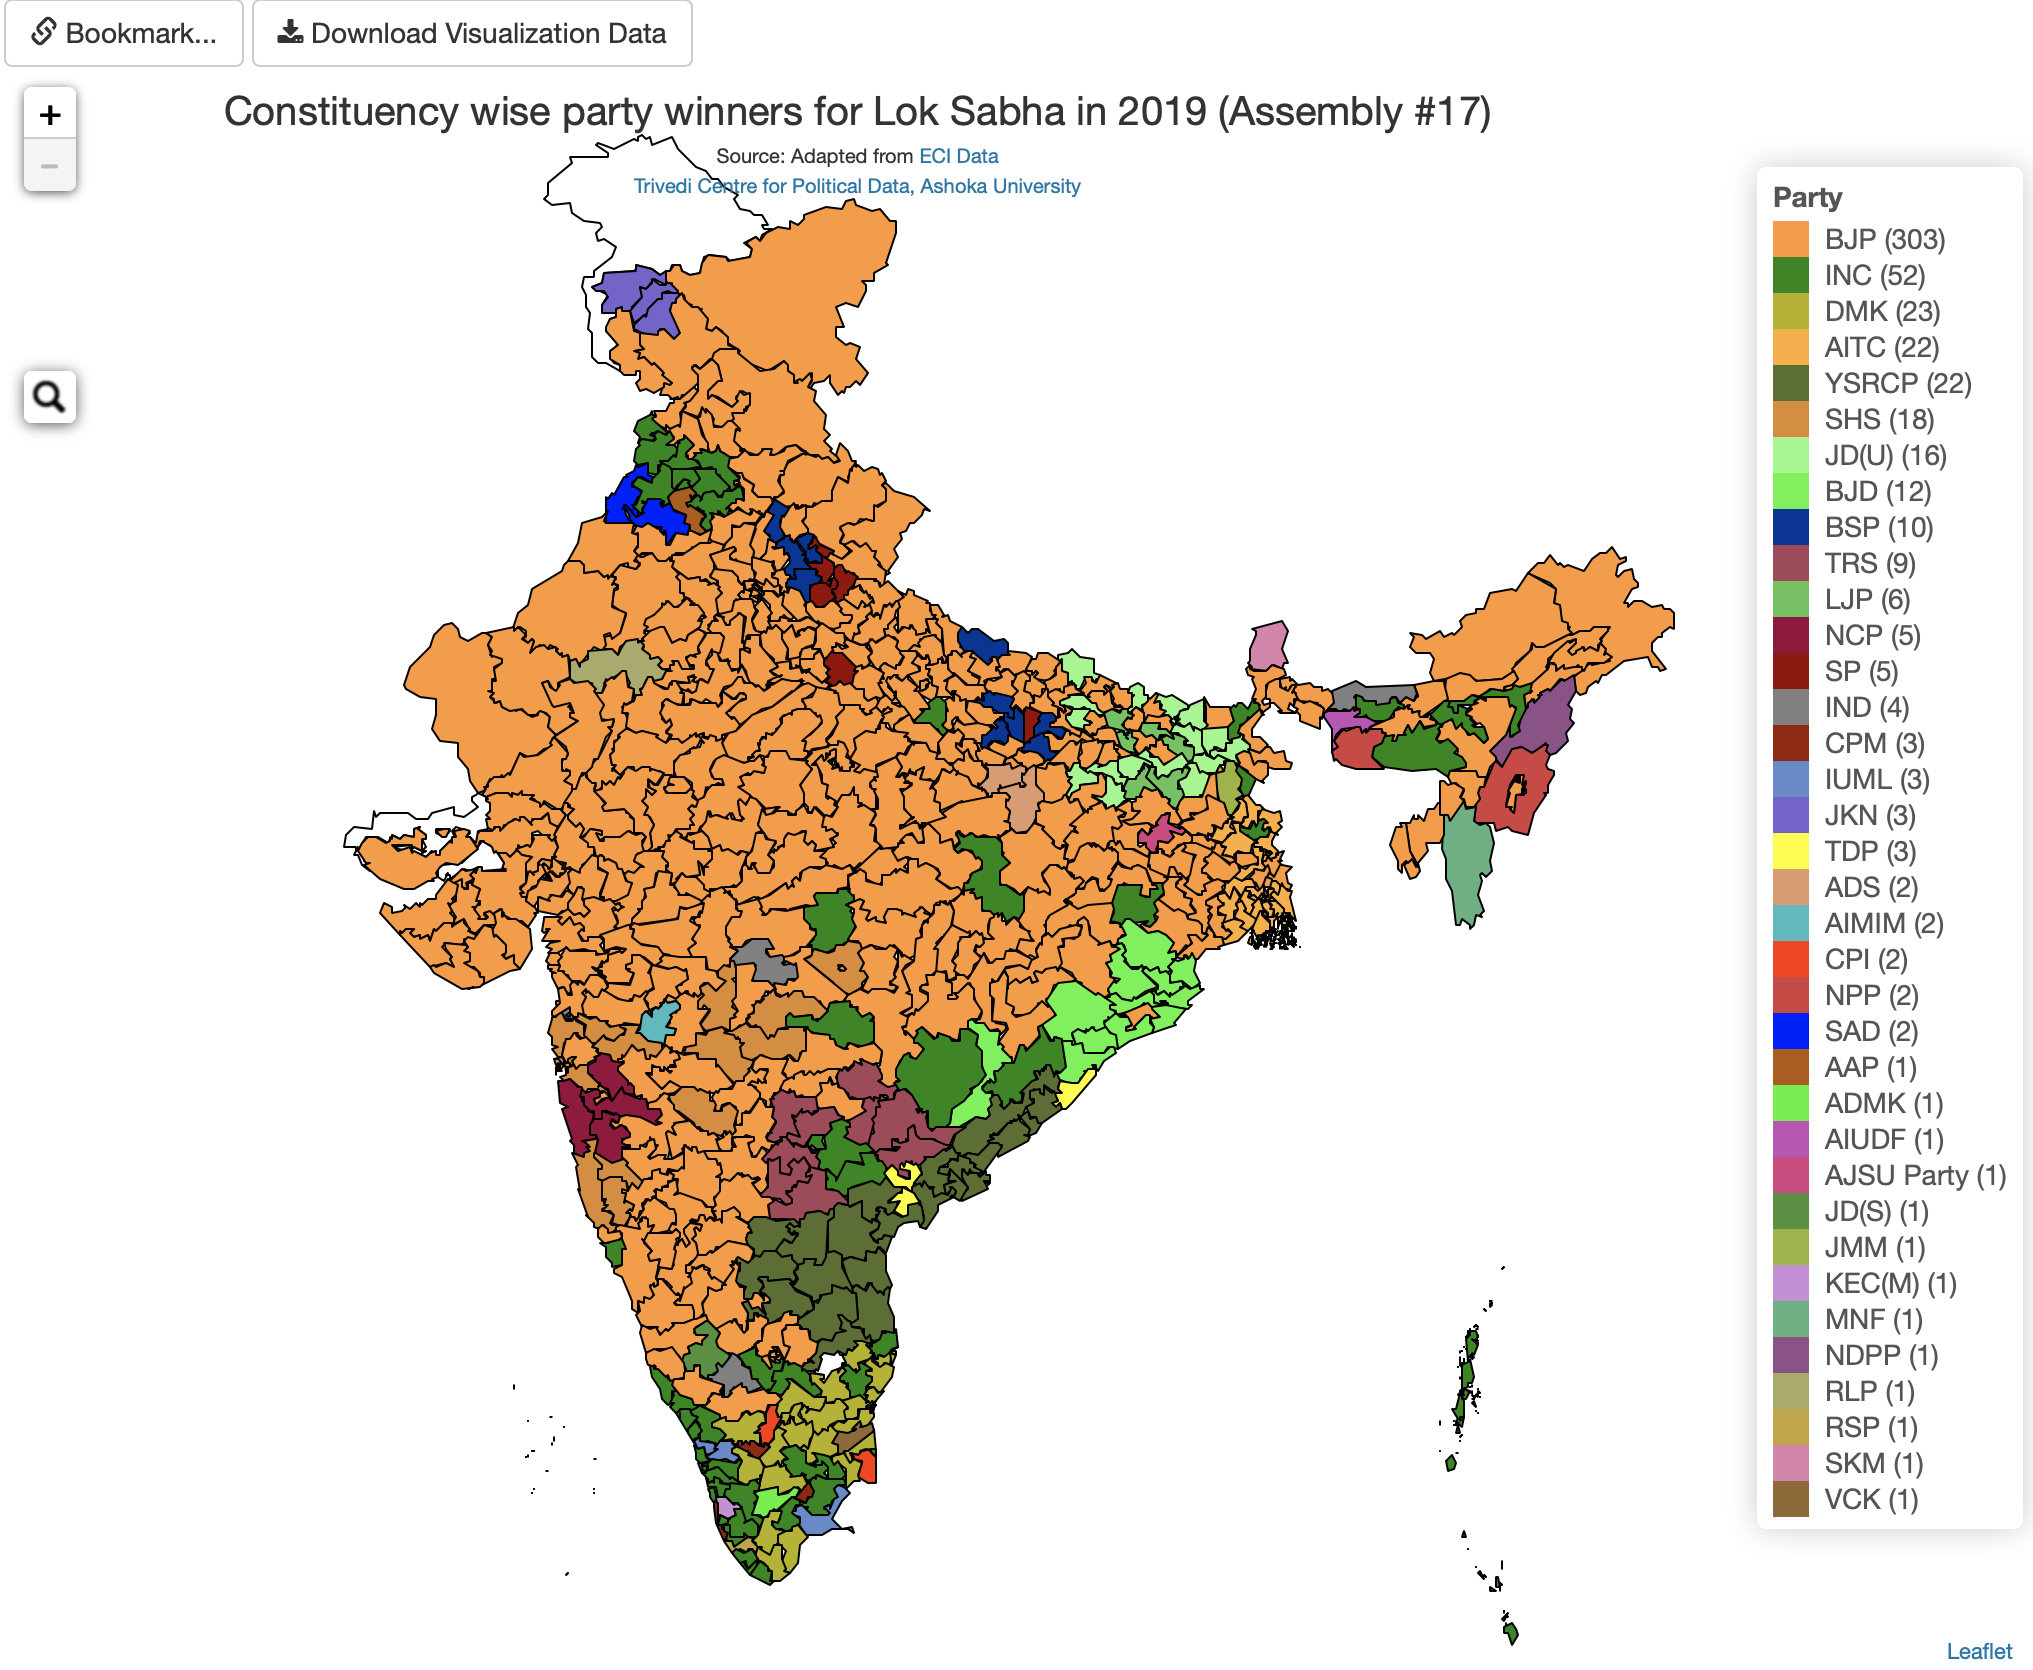
\includegraphics[width=\linewidth]{PartyWinnersMap2019}
 \caption{Visualization of the winning party in the 2019 national elections }
 \label{partyWn}
 \end{figure}
 
 \subsubsection{Incumbency profile}
Indian elections feature candidates who frequently cross over between parties. Candidates' affiliations to parties tend to be based on pragmatic rather than ideological considerations. There is a steady stream of parties splitting and merging, pre-poll and post-poll coalitions, or candidates crossing over from one party to another. There is often an anti-incumbency wave, meaning that a ruling party or legislator may have a disadvantage as voters blame them for poor governance. Assignment of tickets within a party is also an opaque process, with some parties tending to favor loyalists, while others preferring to rotate their candidates. It is therefore very interesting for political scientists to trace the trajectory of individual candidates, and ask who gets nominated, elected, re-nominated, re-elected, etc.

LokDhaba includes a visualization showing career performance of elected members or contestants of a specific assembly. In this visualization, the user can see the complete record of each contestant, such as their current and previous party affiliations and electoral performance. This component is designed to enable the user to view all elected and major-party candidates clustered together by party, while also depicting their party affiliation in the immediately preceding assembly, in order to identify turncoats. Winners and losers are represented by shape, and the shape can be annotated with a single number, either the candidate's number of attempts, or the number of their victories. Upon hovering on a shape, users can view prior contest information and a photograph of the candidate. A search function enables the user to narrow down to a specific person or constituency of interest. Users can also filter down by gender or experience, in order to focus on specific subsets of the candidates.
 
 Fig. \ref{incm_all} shows a snapshot of the winners of the 2019 Parliamentary elections. Fig. \ref{incm_rhl} shows the search for the name "Rahul" and the resulting information on Mr. Rahul Gandhi of the Indian National Congress.
 \begin{figure}
 \centering
 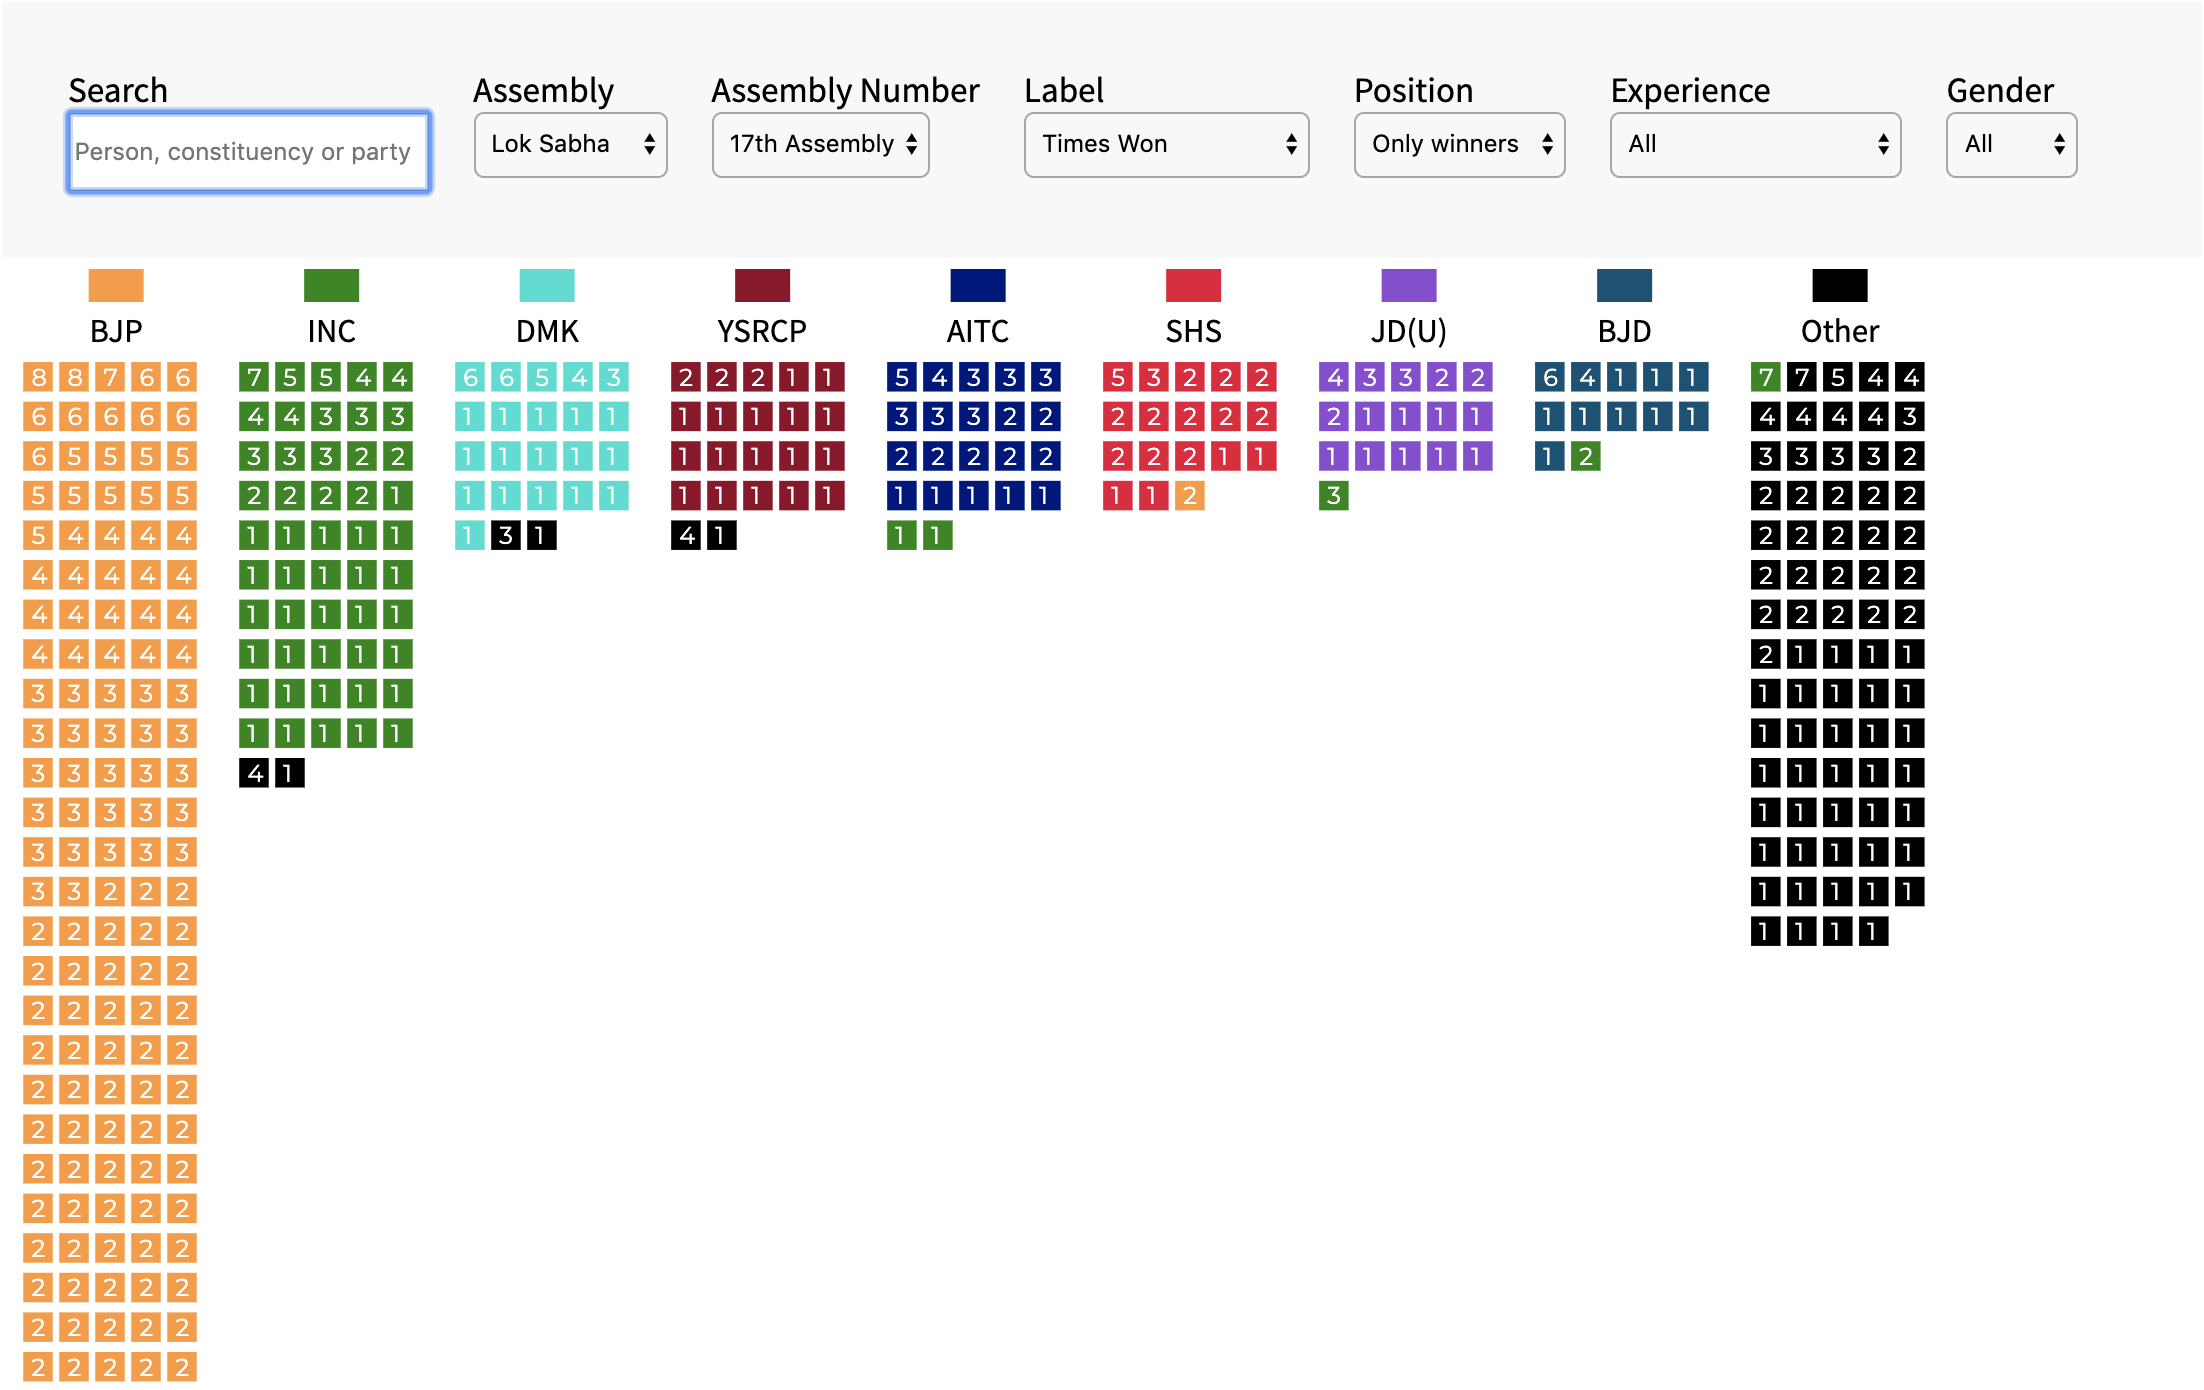
\includegraphics[width=\linewidth]{Incumbency_Profile.png}
 \caption{Incumbency profile of the 2019 national election winners}
 \label{incm_all}
 \end{figure}
 \begin{figure}
 \centering
 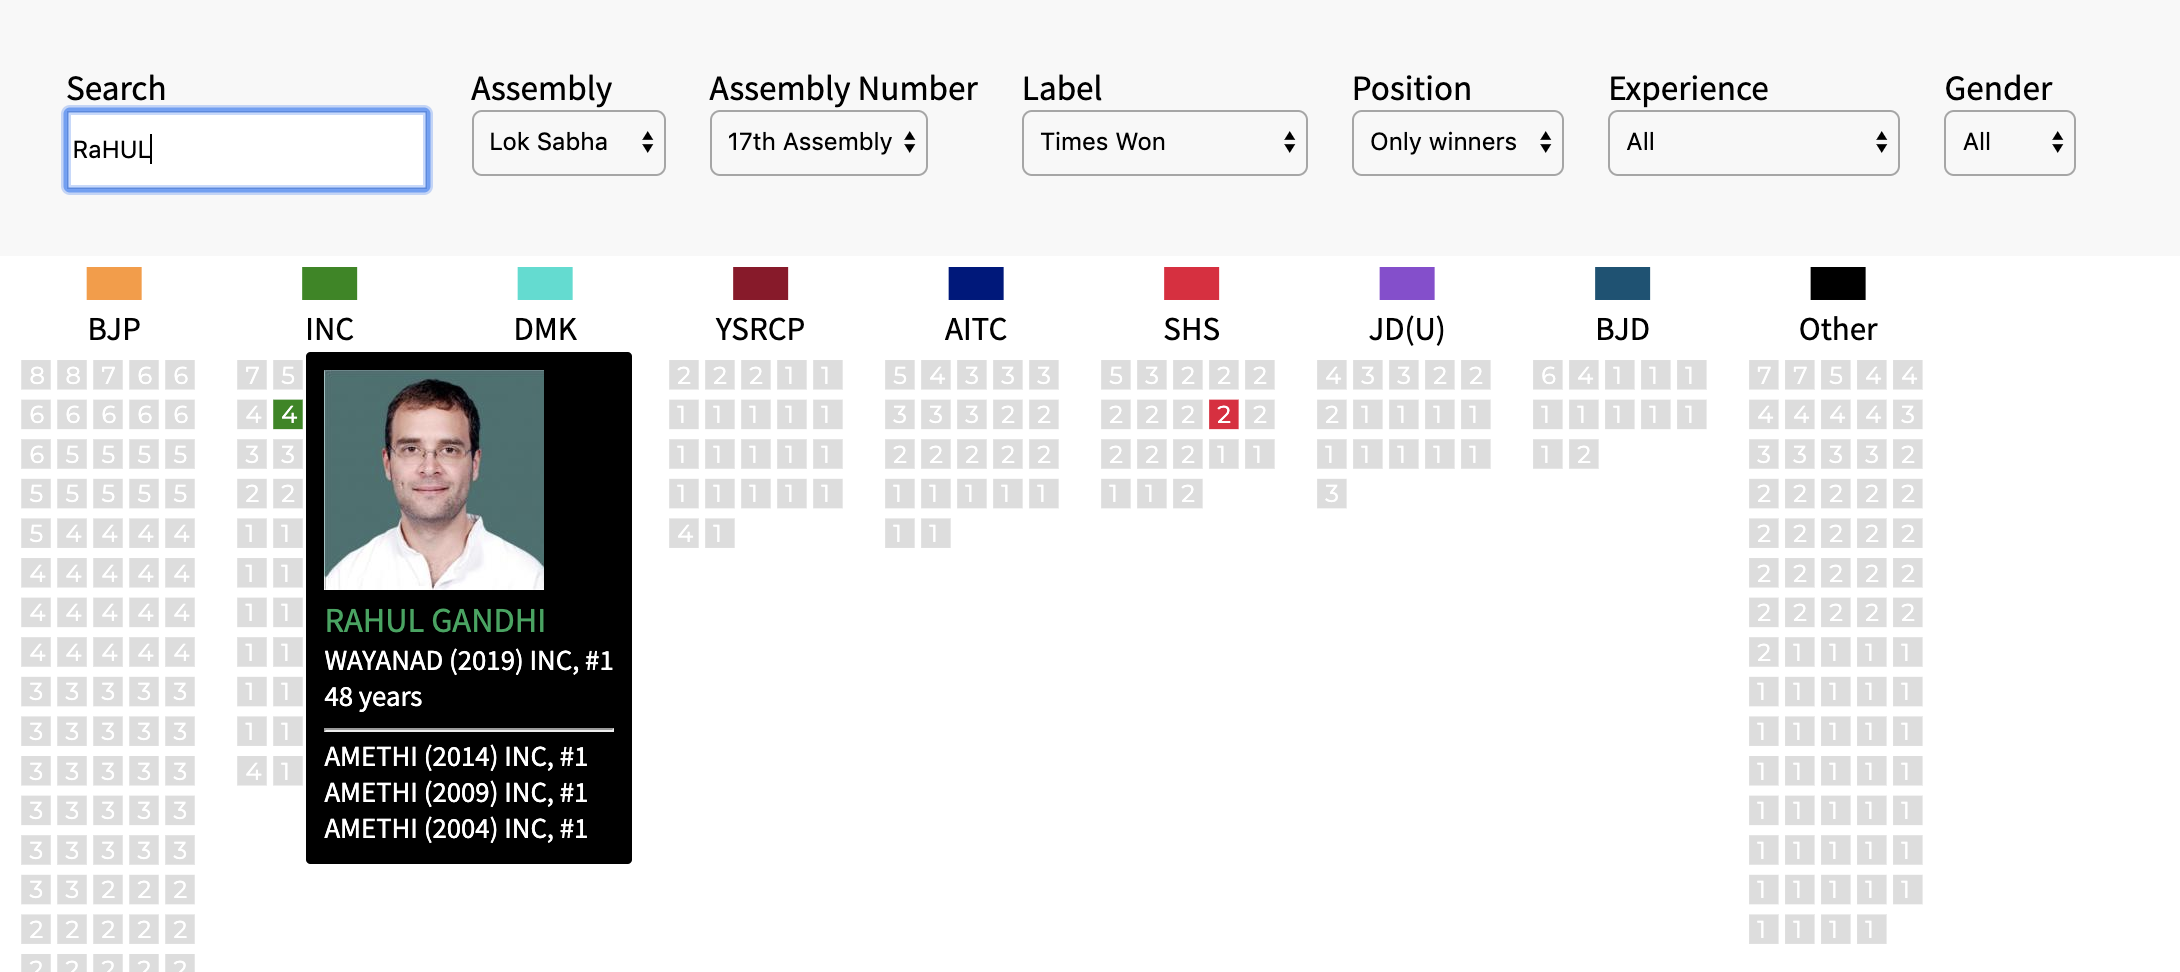
\includegraphics[width=\linewidth]{Incumbency_RG.png}
 \caption{Viewing a candidate's details}
 \label{incm_rhl}
 \end{figure}
 